% !TeX spellcheck = it_IT
\section{Comunicazione Satellitare}

\subsection{Geometria del link satellitare}

\paragraph{Piano orbitale:} Il "cerchio" secondo cui il satellite si muove, generalmente indicato tramite l'inclinazione rispetto all'equatore.

\paragraph{Angolo di Azimuth:} Orientamento rispetto al nord geografico, in senso orario dice dove orientare la stazione di terra per poter ricevere il segnale; vogliamo capire come orientare l'antenna per ricevere o trasmettere nella maniera migliore possibile.

\paragraph{Angolo di elevazione:} Angolo rispetto all'orizzonte; quanto "alzare" il ricevitore.

\paragraph{Angolo di copertura:} Porzione di superficie terrestre visibile da satellite (angolo tridimensionale); quanto terreno copre un satellite, più è lontano maggiore sarà questo angolo.

\paragraph{Lunghezza fisica del link:} Bisogna tenere in conto della distanza dal satellite, in quanto significativa per i tempi di trasmissione, e questa varia in base alla posizione del satellite: sarà minima quanto il satellite è direttamente sopra il ricevitore, sarà massima quando il satellite è all'orizzonte; questo porta a un variare del tempo di propagazione (elevato jitter) durante la durata di connessione al satellite.

\paragraph{Attenuazione in funzione dell'angolo di elevazione:} Un angolo di elevazione molto basso (verso l'orizzonte, link molto lungo) porta a far perdere energia alla trasmissione.

Inoltre, l'attenuazione dipende anche dalla condizione atmosferica, variando, anche significativamente, l'assorbimento del segnale. Ne va tenuto conto durante il calcolo del path loss.

\begin{center}
	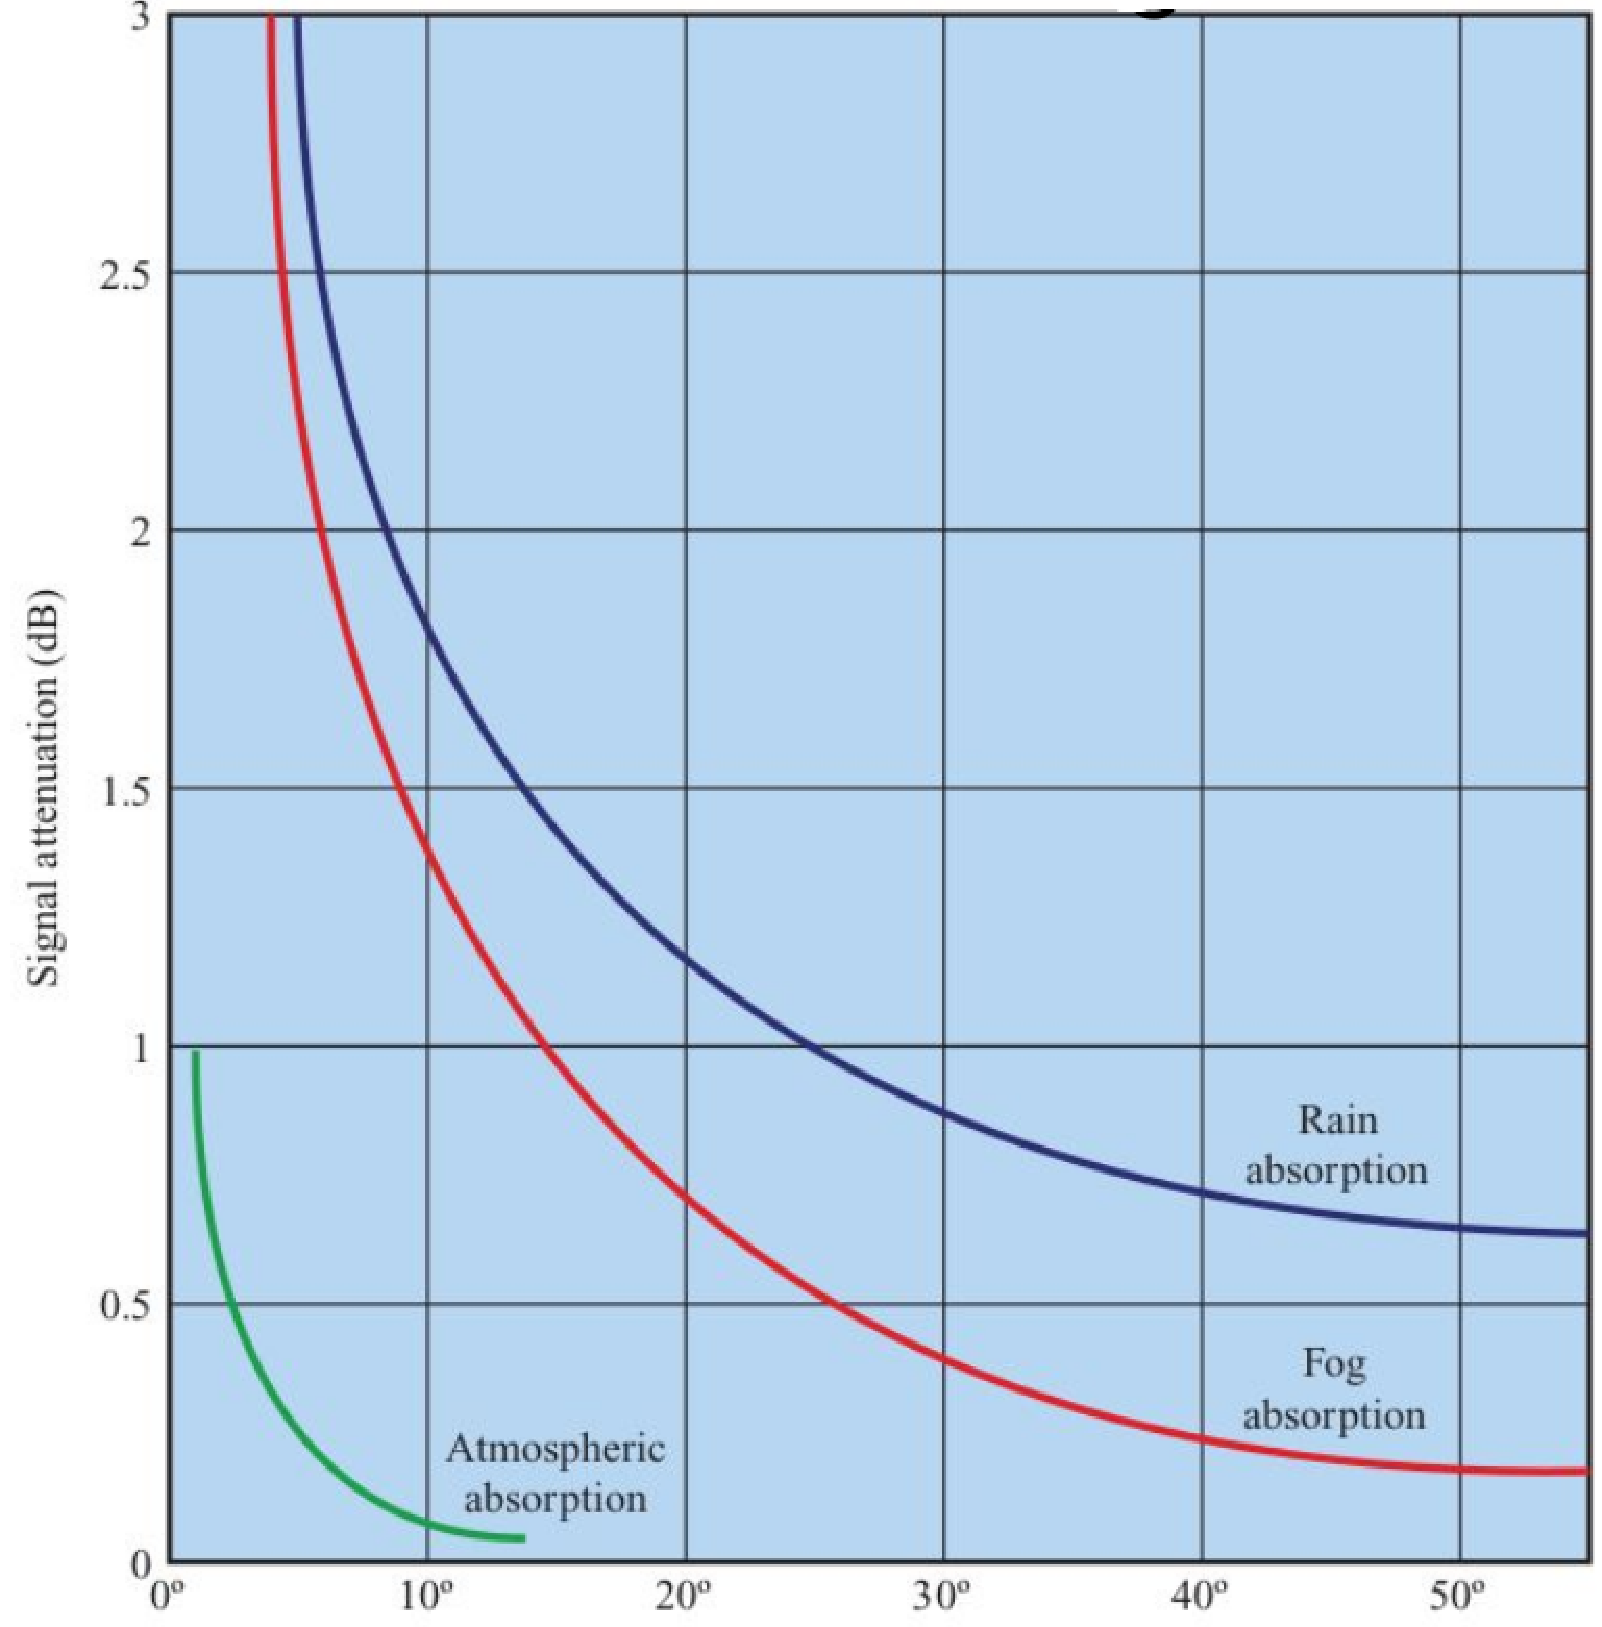
\includegraphics[width=0.65\linewidth]{img/sat/atten}
\end{center}

\subsection{Orbite}

\subsubsection{Geostationary Earth Orbit GEO}

Orbita geostazionaria:
\begin{itemize}
	\item periodo dell'orbita: 24h

	\item visibilità: permanente

	\item angolo di elevazione: fisso

	\item elevata copertura: 3 satelliti separati da 120$^\circ$ coprono la maggior parte delle zone abitate

	\item qualità del segnale bassa a causa della distanza

	\item elevato delay, $\sim 250ms$
\end{itemize}

A circa 35786km di altezza, un satellite ruota alla stessa velocità della Terra, quindi, da una prospettiva "sul terreno", il satellite appare in posizione fissa. 

Questo permette di usare antenne fisse, riducendo costi e complessità a terra, allo stesso tempo avendo una copertura molto elevata (sono lontani, "vedono" molto).

\subsubsection{Low Earth Orbit LEO}

Orbita più vicina alla terra: 
\begin{itemize}
	\item periodo dell'orbita: 1.5-2h

	\item visibilità per passaggio: 15/20 minuti prima che scompaia all'orizzonte

	\item RTT: alcuni ms

	\item copertura: 6000km

	\item ridotto delay per via dell'orbita più bassa

	\item minore potenza di trasmissione e migliore utilizzo dello spettro

	\item La comunicazione tra stazioni terrestri spesso coinvolge più hop tra satelliti (handoff)

	\item garantire la copertura 24/24 richiede un "elevato" numero di satelliti
\end{itemize}

Sempre più rilevanti, in particolare per applicazioni di comunicazione. Sono posizionati a quota tra 160 e 2000km e sorvolano aree diverse a ogni passaggio, con una copertura relativamente limitata. 

I vantaggi sono una bassa latenza e una minor potenza di trasmissione richiesta, al costo di una copertura limitata, di conseguenza richiedendo grandi costellazioni, e una gestione più complessa per quanto riguarda tracciamento, handover e comunicazione tra satelliti.

\subsubsection{Medium Earth Orbit MEO}

Via di mezzo tra LEO e GEO:
\begin{itemize}
	\item periodo dell'orbita: 5-10 ore

	\item visibilità per passaggio: 2-8 ore

	\item RTT: decine di ms

	\item copertura: 12000-15000 km

	\item minori handoff rispetto a LEO

	\item maggiore delay e potenza di propagazione rispetto a LEO, ma significativamente inferiore rispetto a GEO
\end{itemize}

Usato da Global Navigation Satellite System GNSS. RTT, visibilità per passaggio e periodo dell'orbita dipendono (ovviamente) dall'altezza del satellite (abbastanza variabile in questa categoria).

\subsubsection{Costellazione}

Soprattutto nelle orbite LEO e MEO, sono richiesti più satelliti per una copertura continua e globale (o regionale). 

Le costellazioni differiscono per numero di piani orbitali e numero di satelliti. La progettazione della costellazione dipende dai requisiti che si vogliono soddisfare.

\subsection{Architettura}

Sono presenti 3 \textbf{segmenti}:
\begin{itemize}
	\item \textbf{Space} segment
	
    \item \textbf{Ground} segment

	\item \textbf{User} segment
\end{itemize}

\begin{center}
	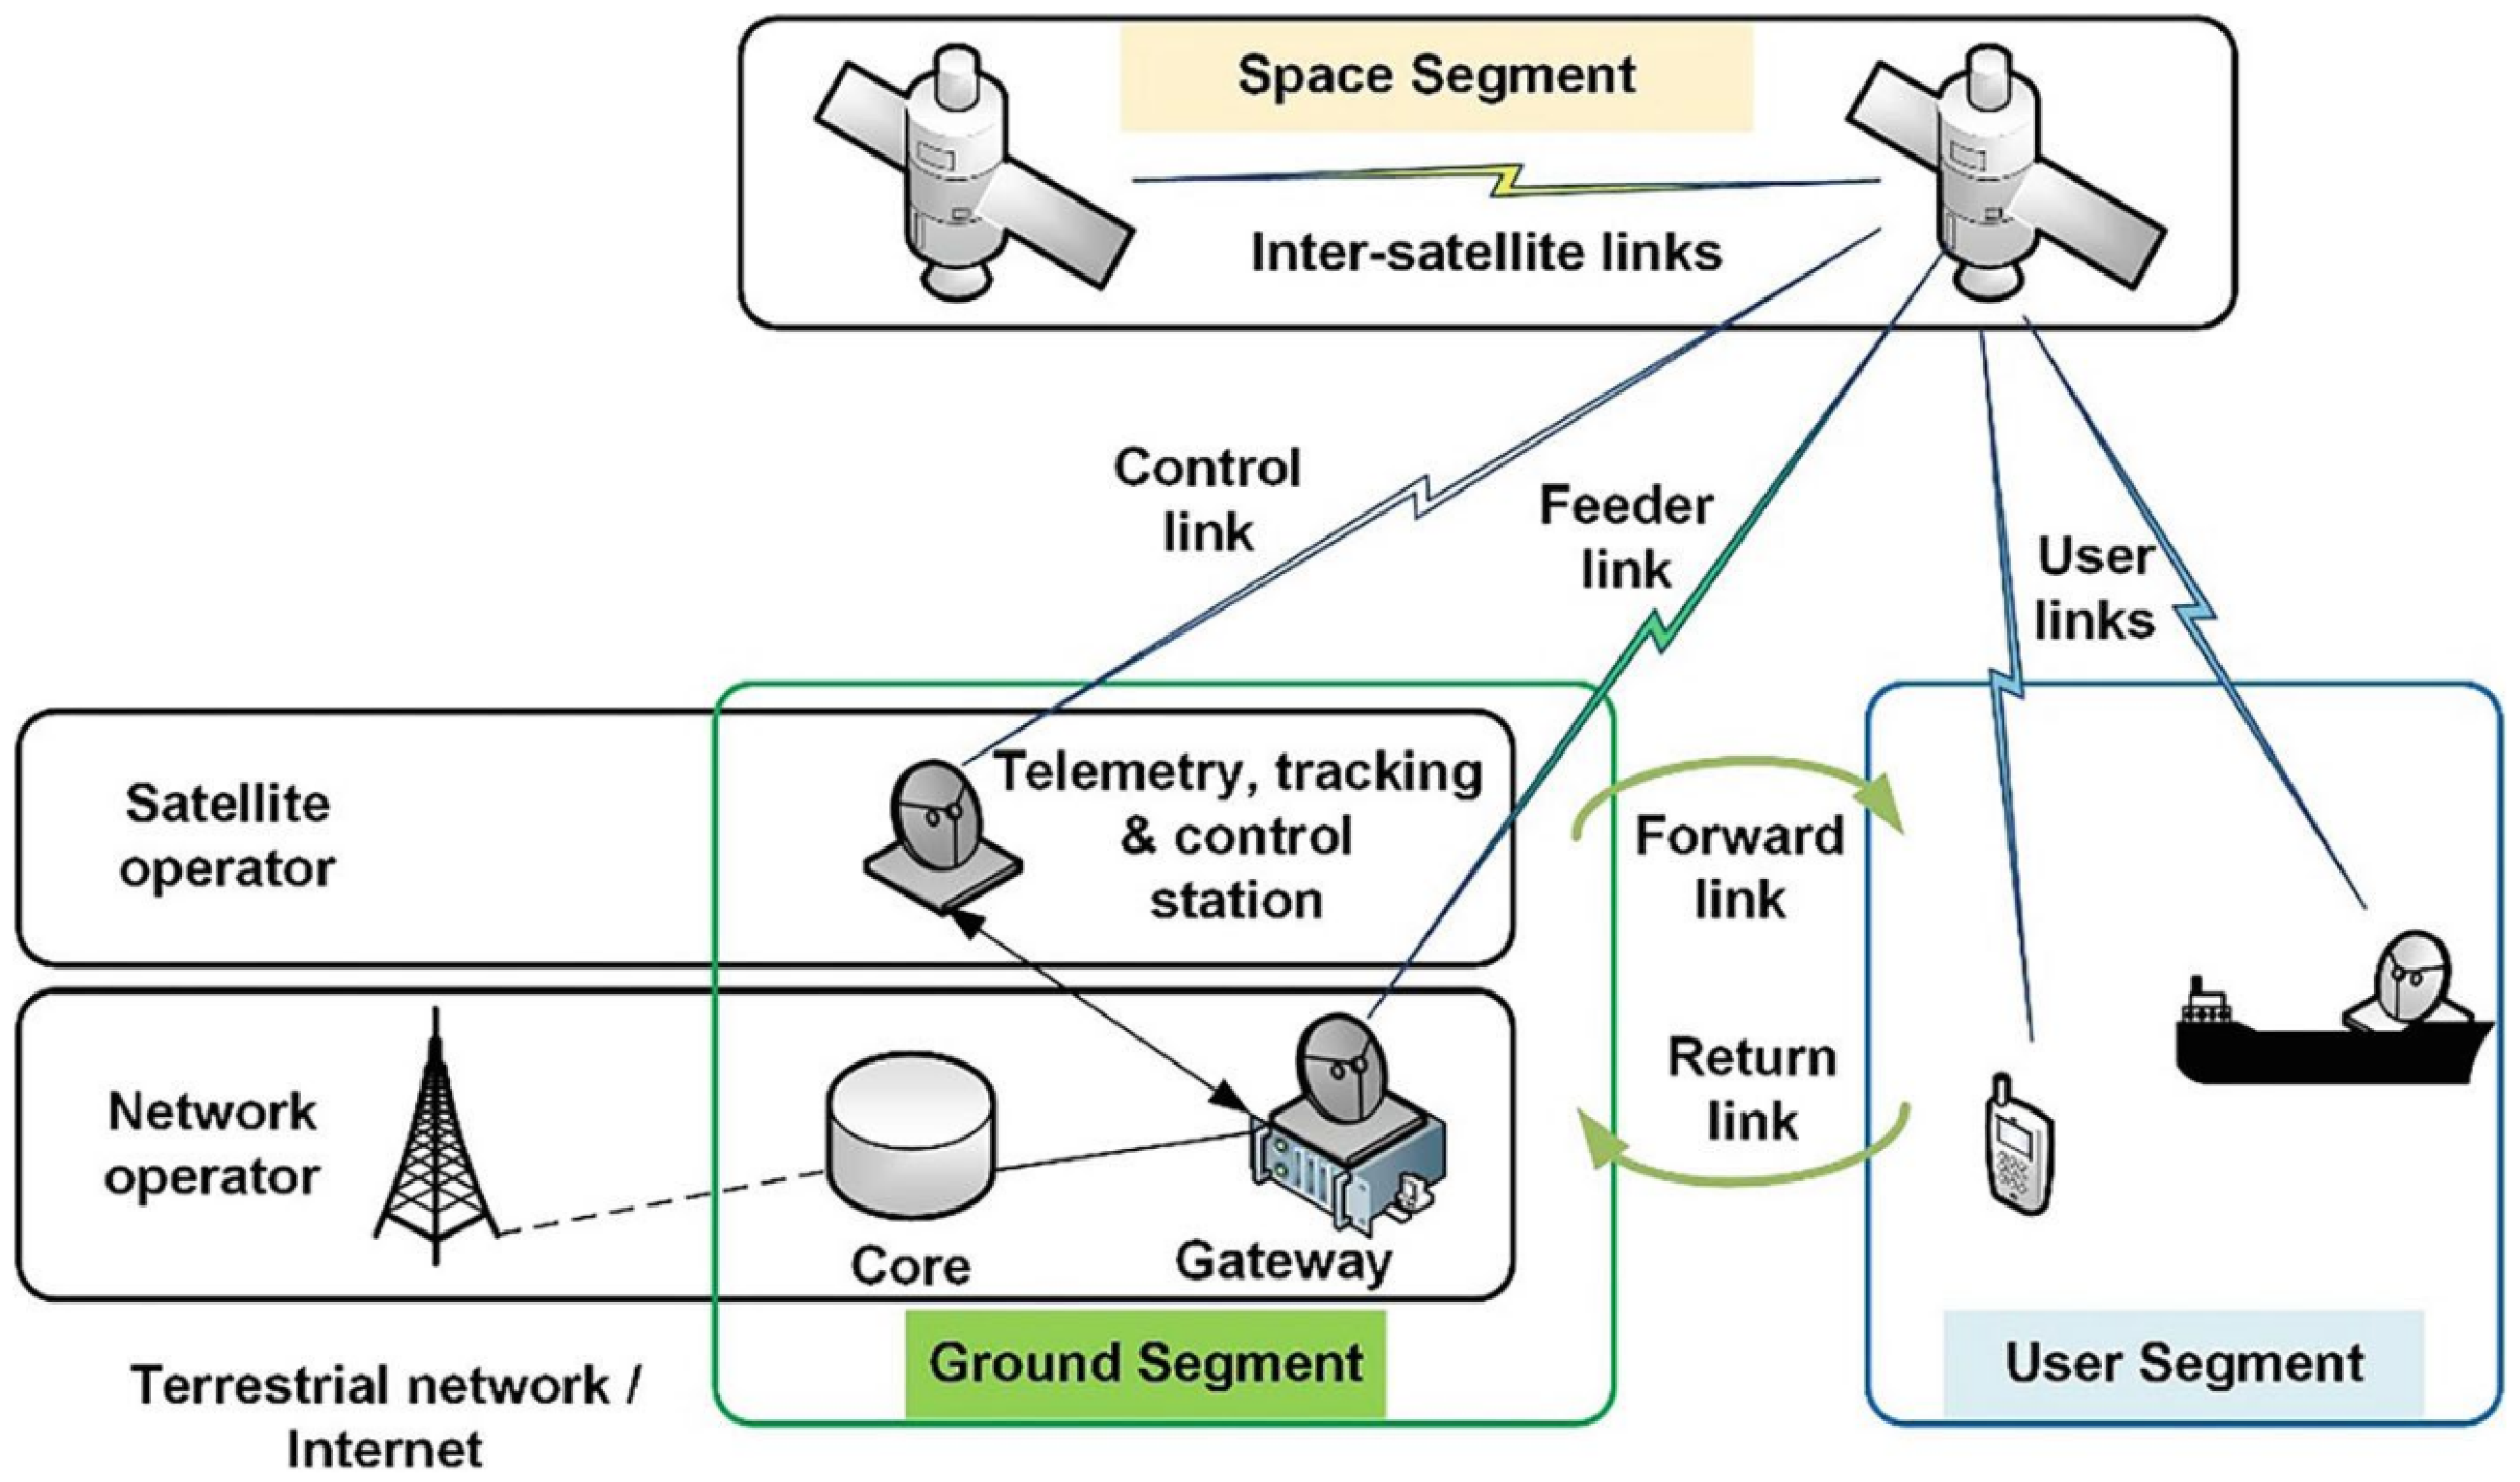
\includegraphics[width=0.7\linewidth]{img/sat/arch}
\end{center}

\paragraph{Space segment:} Contiene i satelliti e le relative costellazioni, con anche la possibilità di avere link inter-satellitare (tramite radio o anche ottici, via laser).

\paragraph{Ground segment:} Contiene la "parte di controllo" del sistema, include il gateway, ovvero ciò che connette le stazioni di terra con i satelliti, oltre che le stazioni di terra e tutto ciò che riguarda controllo, telemetria e tracking.

\paragraph{User segment:} Ovvero gli utenti, utilizzatori dei servizi, possono essere mobili o fixed.

\subsubsection{Allocazione frequenze}
\begin{center}
	\resizebox{\textwidth}{!}{\begin{tabular}{|l|l|l|l|}
			\hline
			\textbf{Satellite band} 
			& \textbf{Frequency range} 
			& \textbf{UL or DL} 
			& \textbf{Satellite services} \\
			\hline
			\multirow{2}{*}{L band} 
			& 1525--1559\,MHz & DL 
			& \multirow{2}{*}{MSS and 5G NTN systems} \\
			& 1626.5--1660.5\,MHz & UL & \\
			\hline
			\multirow{5}{*}{S band} 
			& 1980--2010\,MHz & DL & BSS and 5G NTN systems \\
			& 2170--2200\,MHz & UL & FSS, MSS \\
			& 2500--2520\,MHz & DL & BSS \\
			& 2520--2670\,MHz & DL & FSS, MSS \\
			& 2670--2690\,MHz & UL & \\
			\hline
			\multirow{2}{*}{C band} 
			& 3.7--4.2\,GHz & DL 
			& FSS systems, good rain resilience \\
			& 5.925--6.425\,GHz & UL & \\
			\hline
			\multirow{2}{*}{X band} 
			& 7.25--7.75\,GHz & DL & FSS, MSS maritime \\
			& 7.9--8.4\,GHz   & UL & FSS, MSS \\
			\hline
			\multirow{2}{*}{Ku band} 
			& 10.7--12.75\,GHz & DL 
			& FSS, MSS and BSS systems. \\
			& 14--14.5\,GHz    & UL & \\
			\hline
			\multirow{3}{*}{Ka band} 
			& 17.3--17.7\,GHz & DL 
			& BSS and FSS systems \\
			& 17.7--19.7\,GHz & DL & \\
			& 27.5--29.5\,GHz & UL & \\
			\hline
			\multirow{2}{*}{Q/V band} 
			& 37.5--42.5\,GHz & DL 
			& FSS systems for high throughput services \\
			& 47.2--52.4\,GHz & UL & \\
			\hline
			\multirow{2}{*}{W band} 
			& 71--76\,GHz & DL 
			& FSS system allocations, experimental missions \\
			& 81--86\,GHz & UL & \\
			\hline
	\end{tabular}}
\end{center}

\subsection{Topologie di rete}

\paragraph{Punto-punto:} Il satellite funge da ponte radio tra stazioni e trasmette, l'UL è da stazione a satellite, il DL da satellite a stazione (le due stazioni non si vedono ovviamente). 

Permette un'area di copertura molto maggiore rispetto alla rete wireless terrestre con un elevata banda, ma richiede elevata potenza di trasmissione e ha un delay di propagazione elevato.

\paragraph{Broadcast:} Nell'ambito broadcasting viene sfruttata l'area coperta dal satellite: si può usare un solo satellite per trasmettere a molteplici ricevitori. 

Se la parabola è correttamente orientata verso il satellite, il segnale può essere ricevuto da \textit{tanti} ricevitori.

\paragraph{Mesh:} Si vuole un link tra stazioni usando il satellite come ripetitore, non è necessario un gateway.

\paragraph{Star:} Non esistono link diretti tra stazioni, ma tutto passa tramite il gateway. Ogni stazione comunica, passando dal satellite, con il gateway, il quale provvederà a "smistare".

\paragraph{Hybrid:} Combina Star e Mesh, alcune comunicazioni passano attraverso il gateway ma sono presenti anche link diretti tra stazioni.

Differenze nello scambio di messaggi:
\begin{center}
	\begin{minipage}{0.48\linewidth}
		Star topology:
		\begin{center}
			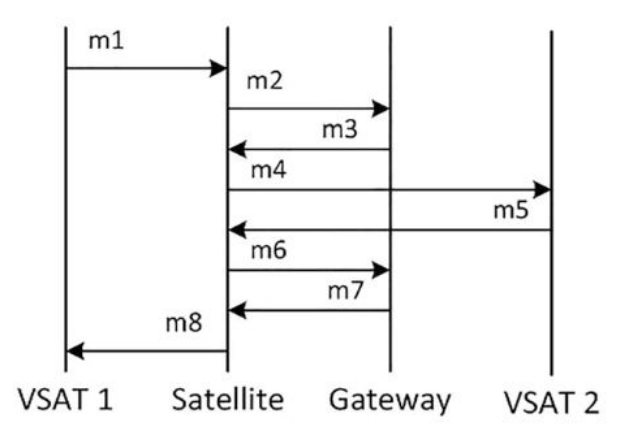
\includegraphics[width=\linewidth]{img/sat/startop}
		\end{center}
	\end{minipage}
	\hfill
	\begin{minipage}{0.48\linewidth}
		Mesh topology:
		\begin{center}
			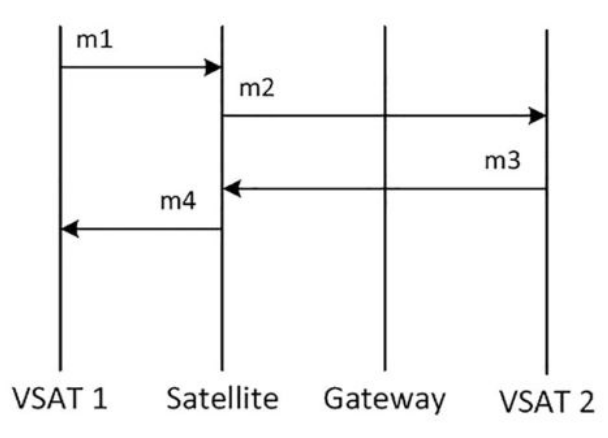
\includegraphics[width=\linewidth]{img/sat/meshtop}
		\end{center}
	\end{minipage}
\end{center}

\subsection{Medium Access Control MAC}

I protocolli MAC per le connessioni satellitari possono essere: 
\begin{itemize}
	\item \textbf{Contention-free}: FDMA, CDMA, TDMA
	
    \item \textbf{Contention-based Random Access}: Slotted RA, Unslotted RA
	
    \item \textit{Demand-based allocations with beam-hopping satellites}
\end{itemize}

\paragraph{TDMA:} Slot di tempo dedicato a ogni trasmittente; per il downlink invece è facile, il satellite manda un \textit{pacchettone} tutto assieme, ogni ricevitore filtrerà ciò che deve leggere.

Richiede una precisa sincronizzazione tra satellite e dispositivo, oltre che un'elevata potenza di trasmissione (non tutti i dispositivi riescono). Complicato in orbite LEO a causa dell'elevata mobilità dei satelliti.

\paragraph{FDMA:} Prima modalità utilizzata per la trasmissione satellitare. Offre una minore efficienza spettrale, quindi può essere combinata con TDMA per migliorare le prestazioni.

Bisogna tenere conto dell'effetto doppler, soprattutto in orbite basse, le velocità modificano le frequenze. 

\paragraph{CDMA:} Usato dalla maggior parte dei sistemi GNSS. Soffre del Near-far problem, molto rilevante se si considerano le distanze in ambito satellitare. Importa relativamente poco per GNSS, richiede solo di scaricare dati.

\paragraph{OFDMA:} Storicamente non molto adottato a causa dell'elevata sensibilità del sistema all'effetto doppler (richiede una certa precisione, impatta di più rispetto a FDMA).

Attualmente utilizzato dalla costellazione Starlink e dai sistemi 5G-NTN (Non Terrestrial Network).

\subsection{Integrated Satellite - Terrestrial Networks and 5G/6G NTN Technology}

Motivazioni: 
\begin{itemize}
	\item migliorare il lancio delle tecnologie 5G/6G anche in aree remote: aree rurali, aerei, navi

	\item continuità di servizio (ubiquitous connectivity): garantire connettività anche in casi di movimento "estremo", posso sempre accedere alla rete cellulare in modo trasparente all'utente

	\item migliorare l'affidabilità della rete, sia in termini di capacità che in caso di catastrofi naturali

	\item aumentare la scalabilità della rete; servizi multicast e broadcast sono difficili da implementare con protocolli unicast, con il satellitare è molto più facile
\end{itemize}

\subsubsection{Architetture possibili}

Come si può integrare la rete satellitare alla rete operatore?

\paragraph{Relay:} Satellite usato per la comunicazione, ma il relay a terra funge da ripetitore del segnale aumentando la qualità del canale. Il segnale può essere combinato BS-satellite, oppure solo relay.

\paragraph{Backhaul:} Costruire la rete di backhaul per raggiungere certe aree (gruppi di gNodeB) potrebbe essere difficile/impossibile: il satellite viene usato come rete di backhaul tra gNodeB e Core Network.

\paragraph{Direct Access:} La rete satellitare offre servizi di connettività direttamente ai dispositivi in single/dual connectivity. Il device può vedere direttamente il satellite.

Un esempio di connessione per utilizzi/dispositivi diversi:
\begin{center}
	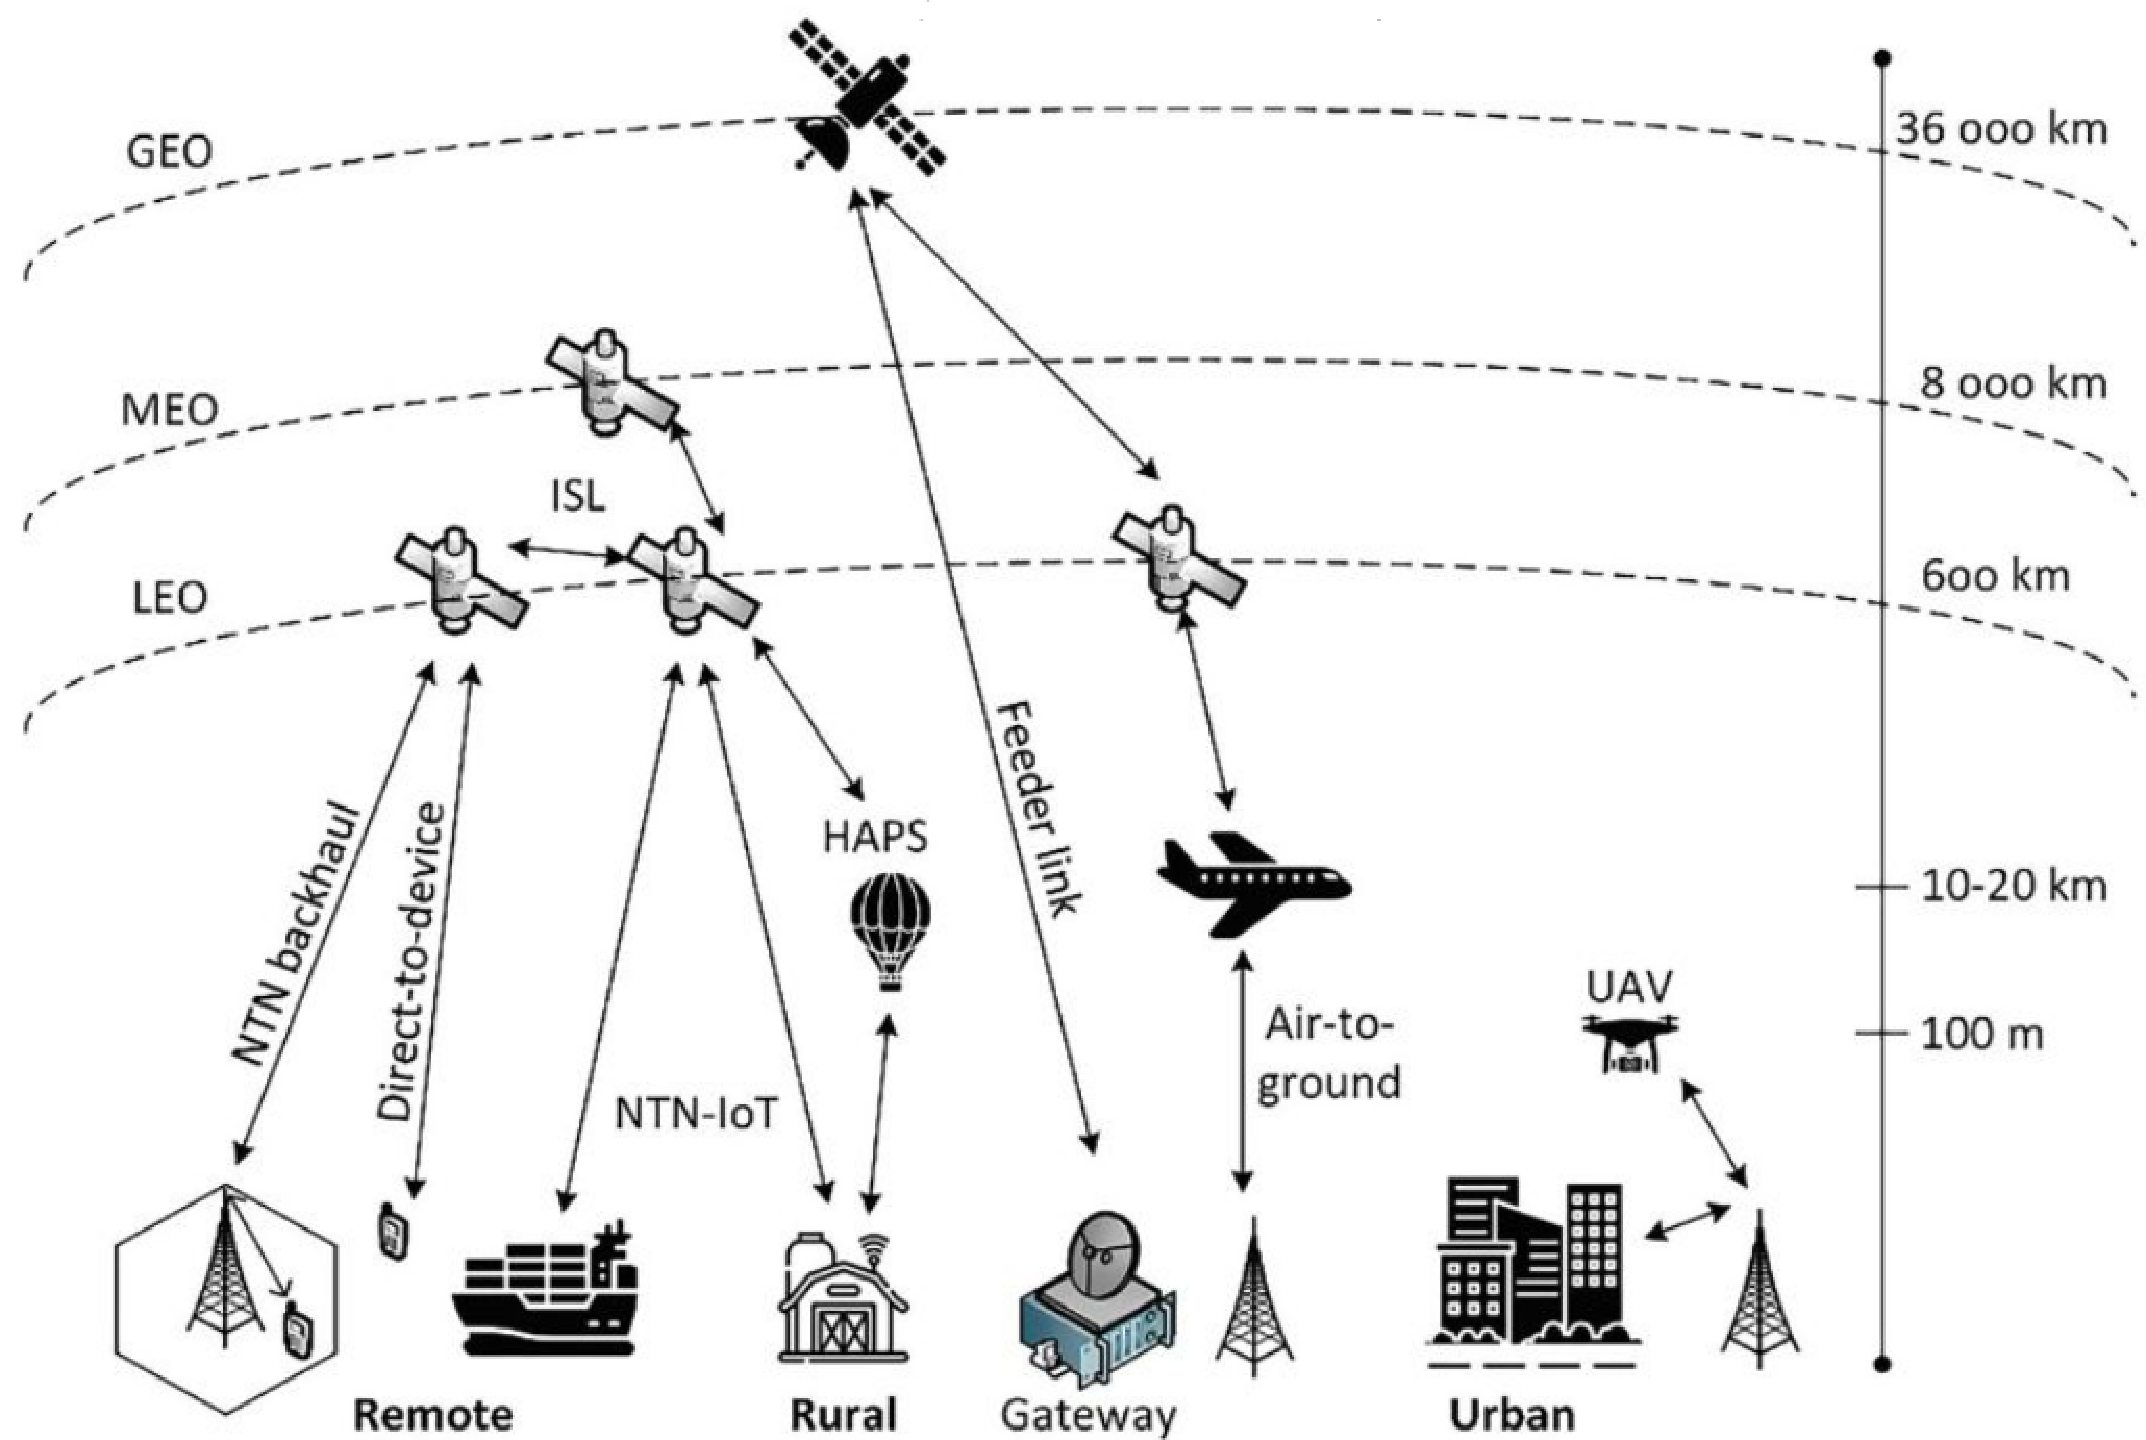
\includegraphics[width=0.98\linewidth]{img/sat/overview}
\end{center}

\subsubsection{Opzioni di integrazione}

\paragraph{NTN Transparent Payload:} Il satellite fa solo da relay, livello fisico, è il gateway che dialoga con la BS.

Questa è la soluzione più semplice, adottata dalle prime release NTN. Il gateway dialoga con gNodeB (con possibili soluzioni proprietarie, non è definita la comunicazione).

\paragraph{NTN Regenerative Payload:} Il satellite implementa lo stack di una gNodeB e ne svolge le funzionalità. 

Permette maggiore flessibilità e utilizzo di Inter-Satellite Link ISL. Il gateway è collegato alla 5G Core. 

\paragraph{NTN Regenerative Payload with Functional Split:} Il satellite svolge solo le funzionalità del modulo distributed unit del gNodeB. 

I livelli di protocolli che il satellite deve implementare dipendono dall'opzione di splitting scelta dall'operatore.

Quindi, in breve, le opzioni per integrare la rete dal punto di visto operatore:
\begin{itemize}
	\item Semplice relay, solo processore a livello fisico
	
    \item tutta la BS
	
    \item solo la parte distribuita
\end{itemize}

% End L24